\documentclass[llncsdoc]{llncs}
%\usepackage[latin1]{inputenc}
\RequirePackage[utf8]{inputenc}
\usepackage{epsfig}
\usepackage{epstopdf}
\usepackage{graphicx}
\usepackage{makeidx}
\usepackage{subfigure}
\usepackage{multirow}
\usepackage{indentfirst}
\usepackage[printonlyused]{acronym}
\usepackage{booktabs}
\usepackage[table]{xcolor}
\definecolor{lightgray}{gray}{0.9}



\usepackage[table]{xcolor}
\usepackage{array}
\usepackage{url}
\newcolumntype{P}[1]{>{\centering\arraybackslash}p{#1}}
\begin{document}
\pagestyle{plain}
\makeatletter
\renewcommand\subsubsection{\@startsection{subsubsection}{2}{\z@}%
	{-18\p@ \@plus -4\p@ \@minus -4\p@}%
	{8\p@ \@plus 4\p@ \@minus 4\p@}%
	{\normalfont\normalsize\bfseries\boldmath
		\rightskip=\z@ \@plus 8em\pretolerance=10000 }}
\DeclareRobustCommand{\rchi}{{\mathpalette\irchi\relax}}
\newcommand{\irchi}[2]{\raisebox{\depth}{$#1\chi$}}
		
\title{Removing Blockcerts' Issuer Hosted Data Dependence}


\author{João Santos\\joao.marques.santos@tecnico.ulisboa.pt}
\institute{Instituto Superior Técnico\\(Advisors: Professors Nuno Santos and David Dias)}
\maketitle
\thispagestyle{plain}


\begin{abstract}

  Something about this
\end{abstract}

\section{Introduction}
We all own credentials that serve as proofs of our proficiency in a given subject. Whether it is a college diploma, or a photography workshop certificate it tends to come in the form of a piece of paper and we usually give it very little use as in the digital age we live in it is not convenient to pass around physical goods. The most common practice is to take a picture of the credential and send to whoever we want to inform about our skills. The obvious problem with that approach is the lack of integrity and identity assurances given how easy it is to forge images.

Furthermore, these diplomas and certificates tend to be very generalised and provide poor personalised information about its owner, for instance a college diploma only states that that individual attended a given course during a period. It gives us no information about the skills he acquired or the activities he was involved in during that time.

Mozilla's Foundation Open Badges movement was created to attend those shortcomings. Open Badges defines a set of mechanism for the issuing, sharing and verification of Badges. A Badge is a digital token that is attributed to an individual by an Issuer as a claim of acquired skill. They obey to a schema that comprises information about the skill (such as a description of the Badge attribution criteria and proof about receiver's the compliance with that criteria), the Issuer, and other useful information such as an expiration date. 

The Open Badges movement also ties up well with the world of reputation systems. While one Badge by itself provides little information, a large number of Badges collected throughout a period of time is a good indicator about an individual's skills and can be used as an indicator to help individuals decide whether to trust each other.

Open Badges has grown a lot in recent years having received wide adoption in online learning platforms such as Moodle, Blackboard that offer native support to Open Badges issuing.

Issuers and receivers can chose where they store their Badges. They can be stored locally and sent, for instance, by email or on online platforms such as Credly, Achievery and Badgelist.

\textbf{Next topics (para completar a intro):}
\begin{itemize}
    \item storing locally makes it hard to share as it is not very scalable
    \item using one of the online platforms has the drawbacks of centralised systems
    \item Blockchain is the most awesome thing ever, so let's use it
    \item Blockcerts brings the best of both worlds. It implements the Open Badges Standard and harnesses the power of the Bitcoin blockchain.
    \item Even though they are using blockchain there still exists a reliance on Issuer hosted data, which is desirable to remove
\end{itemize}


\section{Goals}
\label{sec:goals}

The goal of this project is to contribute to the Blockcerts community project in two fronts:
 
\begin{itemize}
    \item Improve the certificate revocation process
    \item Reduce the dependence on Issuer hosted data
\end{itemize} 
 

\section{Related Work}
\subsection{Status of Certification}
Formal learning entities, like schools, universities and enterprises are known for certifying individuals who partake in their courses. Those certificates are usually physical goods, printed in paper, stamped by the certifying entity, and that stamp is what confirms its authenticity. Unfortunately in recent years several cases of certificate forgery, \cite{SEWARD:2007wu}, \cite{HARRISON:2016uq}, have come to light. Poor certificate verification mechanisms would not constitute a serious problem if said certificates had no real importance, but that is not the case. For a lot of professional careers, certification is a decisive factor on whether an individual should be hired, or what his salary should be. For that reason, certification is something that should be taken seriously. In most cases it is enough to simply list a certificate on our CV and no one will confirm its authenticity since that would require the hiring party to contact the entity who emitted the certificate. That is a laborious and expensive process (there are companies who specialise in professional credentials checking, \cite{Equifax:vn}), especially if we consider places with a high hiring rate, and companies simply can not afford to do it. What is needed is a better way to issue and verify certificates.

\subsubsection{The First Steps Towards Skills Certificates Verification and The Shortcomings of Current Systems}

In recent years Massive Open Online Courses (MOOCs), \cite{Ch:2013ws} have received widespread adoption. MOOCs are free online learning programs usually composed of videos and interactive platforms to teach and test students. There a number of providers and they tend to be associated with universities or companies, Coursera (Stanford), Khan Academy, Udacity (Georgia Institute of Technology, Google, Facebook, Nvidia), Lynda.com. One of the main MOOC providers is edX, which is associated with MIT, Harvard University and more recently, Instituto Superior Técnico. The reason why edX is relevant in this subject is because it is one the MOOC providers that give its participants the ability to receive certificates upon completing a course.

Since 2015, for a small fee, edX offers its participants two types of certificates, Verified Track Certificates that certify a participant on a particular course and XSeries Certificates that confirm a user has received a Verified Track Certificate for each course in a Series of courses. Given that an XSeries Certificate is no more than a set of Verified Track Certificates we are going to focus on the latter. A Verified Track Certificate contains information about the participant (whose identity is automatically verified using a webcam and a copy of a government issued ID) name of the course, the edX partner institution responsible for the course (usually a university), names and signatures of members of the course's team, an issuing date and more importantly a URL that anyone can visit that verifies the authenticity of the certificate. Coursera and Udacity offer similar verified certificates. 

Having these verifiable certificates is an important and welcome improvement to the traditional paper certificate that is still used today in a lot of cases however it still falls short of an ideal system since the ability to verify a certificate is entirely dependent on the certificate issuer, in this case, the Mook platform. If the platforms ceases to exist or for some reason loses track of a specific certificate its receiver is no longer able to prove the claim that he complete a given course. This is the underlying problem of relying on centralised systems, they constitute a single point of failure. Further, in this section we are going to see how Blockchain technology can be used to mitigate this issue.


So far we have been discussing the ways certificates are issued and verified, now we will be delving on the relevance of their content and relevance and for that let us use two students, Alice and Bob, as example. Alice and Bob both attended the same university, Instituto Superior Técnico, in the same period, 2012 to 2017 and pursued the same degree, Computer Science, but that is where their academical life similarities end. 

In her first year Alice joined the IEEE-IST Student Branch, a student group where she gained a lot of experience in organising events such as conferences and technical lectures as well as team management skills. She also participated in of workshops about topics not related to her degree, such as photography and sewing, and received certificates from taking those workshops. As a very proactive IEEE member who sponsored innovative programs, Alice was awarded with the IEEE Student Enterprise Award, and received a certificate, signed by the IEEE President, delivered to her residence by mail.

Bob, on the other hand, was always very attracted to programming so he joined a programmer's student group and throughout the five years of his course he participated in a lot of programming competitions and hackathons, having won multiple trophies. Bob was also very active member on the Stack Overflow\footnote{The largest online programmers community, where users can post and answer technical questions.},\cite{stackoverflowcom:RUwG9opz}, contributing a lot to the community in programming problems related to the C and Python programming languages, those contributions earned him the Refiner\footnote{StackOverflow badge awarded to those who answer more than 50 questions in 12 hours} and Mortarboard \footnote{StackOverflow badge awarded to those who received the daily maximum reputation score in a day} badges,\cite{Anonymous:V-xylGNf}. As the programming enthusiast that Bob is he was also very active on HackerRank\footnote{www.hackerrank.com, a website where users can enrol in programming challenges that give them badges}, having participated in a lot of challenges and having won the Algorithms and Machine Learning badge.

Clearly Alice and Bob are two people with very different skill sets. While Alice has acquired a broader set of capabilities, Bob focused on a very particular skill set, however they will both receive the exact same university certificate. The most important document regarding formal education fails at distinguishing two people who are nothing alike.

Furthermore, there are underlying problems with the tokens (awards, certificates, badges) Alice and Bob collected throughout their tenure at university. Alice's paper certificates and awards have all the problems stated in the beginning of this section (expensive to share and verify) and Bob's badges are only relevant in the ecosystem they were issued in because even though StackOverflow and HackerRank's badges provide information about a similar skill set (programming) they are not interchangeable, meaning that StackOverflow does not understand HackerRank's badges and vice-versa. Badges are actually a very good way of providing very granular information about a users skills, as they provide information about individual skills, rather than about general areas of knowledge. Moreover, the gamification techniques, \cite{Deterding:2012wi}, behind badge reward mechanisms have been shown to have positive outcomes in motivating participants to pursue desirable behaviours in a given ecosystem, \cite{Hamari:2013ju}, \cite{Ibanez:2014cs}.

It would be desirable for Bob's reputation \footnote{Reputation to be understood as the amount of badges} in one of these platforms could contribute to his reputation in the other one. This is the problem of information silos. 

Many of the identity and reputation systems (Google, Facebook, Amazon) we use today are extremely atomic in the sense that the information collected by each one is not shared, or even compatible, to the one that is stored in other systems. What this creates, for each user, is a set of incomplete identities. 

A positive step in the direction of creating a system where user's skills are holistically represented is LinkedIn's skill endorsement functionality \footnote{https://www.linkedin.com/help/linkedin/answer/31888/skill-endorsements-overview?lang=en}. Users can endorse other users on arbitrary skills. Those endorsements are displayed on the user's page with the name of the skill and number and names of users who have endorsed. Having an identity associated with an endorsement in an important feature as it helps other users decide whether to value that endorsement (a person will value an endorsement if he trusts the judgement of the endorsers, the same logic applies to university diplomas, given that a diploma is nothing more than a university endorsing an individual on the set of skills he was taught and then employers can decide whether to trust in the endorsement that university made). Another important feature of this endorsement system is that gives users a lot of control over the endorsements they receive and give. A user has the option to retract endorsements he made and to hide endorsements he received from someone. There is also the option to disable endorsements all together.

LinkedIn's endorsement mechanism is an improvement over other digital certification mechanisms, such as edX (LinkedIn even allows for edX certificates to be embedded in a user's profile), in the sense that it adds a lot of functionality and flexibility, however it also consists on an information silo. Even though users have a lot of control over what the website displays about them, LinkedIn always has the final word. If the website ceases to exist, the entire user's reputation that might have taken years to build vanishes.

What is needed is a system that takes the best features of all the above, ease of validation, high granularity, interoperability, gamification, decentralisation and combines them into one cohesive ecosystem. This is exactly what Open Badges aims to achieve.

\subsubsection{Open Badges}

Open Badges are a way to know about an individual's achievements (and skills) by encoding relevant information about each achievement in a digital file. An Open Badge is just like a certificate, only instead of being a PDF file, piece of paper, or a digital token that lives on a website (and is only relevant in the context of that website) is a file that contains relevant information about a certain achievement or skill, has the capability of being easily verifiable and can be linked to other Open Badges issued by different entities. For a file to be considered an Open Badge it has to obey the Open Badges specification, \cite{Anonymous:B6vGjZ5Q} which defines mechanisms for how information about accomplishments and skills should be wrapped (a schema) and packed into portable image files, badges, and the infrastructure for the validation of those badges.

An Open Badge is a JSON-LD\footnote{JSON for Linked Data, allows for files to link to reference each other} file that comprises the following information about who issued the badge(Issuer), who received it (Receiver) and about its meaning(Assertion):
\begin{itemize}
\item \textbf{Issuer:} An Issuer is identified by a Profile class object that contains the Issuer's ID, the name, email and URL. It can also contain a Public Key if the issuer wishes to sign its certificates.
\item \textbf{Receiver:} The Receiver is identified by an Identity object that contains an identity field, that can be an Email for instance. This field can be plain text string, however that is not advised due to privacy issues. Instead, the identity field can be a hash of the identity.
\item \textbf{Assertion:} This is the object that provides context about the achievement or skill. It contains an ID, a Badge class object (that describes the type of badge being attributed), a Verification Object (that has instructions for verification) and the issuing date. It can also contain an expiration date and an Evidence object that gives context to the tasks the receiver completed in order to be awarded the badge.
\end{itemize}
Since the badges are JSON-LD files they can reference other badges' fields, for instance an Evidence field in a badge can be a reference (URL) to the Evidence object that lives in another badge.
Open Badges allow for extension, meaning that each Issuer is free to customise its badges in order to fulfill its needs.
Badges can be Issued by anyone by using what is called a Bakery, which is essentially a program that receives the information listed above and outputs a badge. This output can come in one of two forms. It can be a file, JSON-LD, that the issuer hosts (on a web server controlled by him and shares a link, URL, to it with the receiver) or it can be a PNG image file that contains the JSON-LD embedded in it. In the first approach the Issuer has control over the badge and the verification and authenticity of the badge is proven because the Issuer is the one hosting the badge (so anyone who visits the URL and sees that the badge exists has an automatic confirmation of its existence). This verification approach is similar to the one used by edX. In the second approach the receiver is the one who controls the badge and the way to store it is to use a Wallet, an application designed to keep Open Badges. In order to verify the authenticity of the badge, the badge must have been signed by the Issuer. The most popular Wallet application is the Mozilla Backpack which allows not only for users to store their badges (so far it has more than 1 million badges stored) but also to share them across the web with any applications that have Open Badges support.

One can now see that the Mozilla Backpack was a great improvement as far as certification goes. It implements a standard, Open Badges, that has well-defined mechanisms of verification, that has a high semantic granularity, that makes use of the benefits of gamification, that allows for a high degree of interoperability. 

The Mozilla Backpack is a centralised system that stores badges it solves the interoperability problem that occurs in information silos, however a user is still dependent on Mozilla's goodwill to continue storing their badges. Granted that users can always keep local copies of their badges, but if they don't and the Backpack platform ceases to exist there will be no record of those badges, because no one will be keeping track. Up until recent years this problem would not have an apparent solution. But that is no longer the case as Blockchain technology has paved the way for truly decentralised applications. Decentralisation is the key for certification and Blockcerts is defining the way blockchain technology can be used with Open Badges, more on that in \ref{rel:blockcerts} but first let us explore the blockchain.


\subsection{How the Blockchain Paved The Way For Decentralisation}
Blockchain technology was made popular with the creation of the Bitcoin \cite{Anonymous:JOJGrvgg}, in 2009. Bitcoin was the first truly decentralised crypto-currency, it uses cryptographic properties to solve the Double-spending problem and allows for parties to engage in transactions without having to trust each other. On backbone of Bitcoin is the blockchain which is a distributed ledger that keeps track of every valid transaction that ever took place in the network. Transactions are validated and packed into blocks that are then added to the ledger by nodes (miners) that run a consensus protocol, proof-of-work in the case of Bitcoin. Bitcoin's blockchain has full auditability \footnote{meaning that any node can verify the validity of any transaction} and correctness \footnote{meaning that all the transactions on the longer chain are valid}.

Following Bitcoin's success, a large and active community has emerged and worked on a lot of modifications and extensions to the original protocol to improve some of Bitcoin's shortcomings like performance, introduce new consensus protocols, add new features. These modifications and extensions, which are usually forks of Bitcoin or abstractions that sit on top of existing blockchains, are called "alt-coins", \cite{Bonneau:2015ema}.

One of the shortcomings of Bitcoin was the lack of contract customisation as while it did allow for parties to create some rules regarding a given transaction (such as requiring a third party to approve the transaction) doing so required learning a not very intuitive scripting language and functionality was extremely limited. In other words, it only allowed for a very simple form of smart contracts \footnote{smart-contracts are programs that run on the blockchain and allow for the creation of special transaction rules}. Ethereum is a crypto-currency blockchain, similar to Bitcoin in many ways, that is a smart contract and decentralised application platform. It has a Turing complete programming language which allows for users to create distributed applications while making use of the features of the blockchain.

\subsection{Bitcoin}

\subsubsection{Historical Context}

 Since the 1980's that there had been proposals for crypto-currency systems and in 2005 for decentralised consensus protocols. The proposed crypto-currency systems were never widely adopted due to the need of a centralised platform, as for the decentralised consensus protocols, they never became a reality as it was unclear how to carry out the implementation.
 Bitcoin's white paper,\cite{Anonymous:JOJGrvgg}, was published in 2009 by Satoshi Nakamoto (a pseudonym) and it was the first successful implementation of a decentralised cryptocurrency system.
 
 The technical breakthrough it provided was the implementation of a blockchain, a distributed ledger that keeps track of transactions. 
 \subsubsection{Technical Breakthrough}
 Bitcoin proposed an alternative mode of establishing trust between transacting parties. On traditional financial transaction systems, such as banks, two transacting entities have trust on a centralised element, the bank. Let us look at the example of a normal wire-transfer. User A sends money to user B. Both A and B are confident that the bank will withdraw the right amount of money from A's account and place that same amount in B's account. In this traditional trust model the bank is an essential entity in the process as it constitutes the only source of trust between the two transacting parties. Bitcoin's approach is different. Instead of asking the two parties to trust each other, it uses a proof-of-work system whose cryptographic properties are enough to assure transactional correctness as long as honest nodes control the majority of the CPU power of the network.
 
 An electronic currency is nothing more than a piece of digital data and one of the features of digital data is their easy replication. For that reason, an issue that an electronic currency has to tackle is the double spending problem. That is, ensuring that a given node is not able to spend the same token\footnote{coin, a unit of digital currency} more than once. The way to solve this problem without resorting to a centralised system is to create a ledger of transactions and get all the nodes to agree on the content of that ledger. 
 To that end, a consensus protocol is used, the Bitcoin consensus protocol, also known as the Nakamoto Consensus if based on a proof-of-work.
 
 \subsubsection{Transactions and Proof-of-Work}
 A Bitcoin transaction consists on nodes exchanging unspent coins and is identified by chain of digital signatures. To complete a transaction the sending node digitally a hash that identifies the past transaction and the public key of the next owner. This ensures that each transaction is linked to the ones preceding it, creating a chain.
 The next key challenge is getting all the nodes to agree on the set of past transactions, in order to prevent double-spending.
 To that end transactions are packed into blocks, and added to an append-only data structure, the blockchain.
 
 To add a block to the blockchain, nodes have to mine the block and the way to do that is to solve a mathematical challenge with a pre-defined difficulty level. The first node to solve that challenge mines the block, permanently adding it to the Blockchain. Each time a node mines a block, a new Bitcoin (coin) is created and given to that node. This constitutes an incentive for nodes to mine. The algorithm is designed to automatically adjust the challenger's difficulty in order to regulate the currency issuing rate.
 
 All the mined blocks are made of transactions that are linked to each other, which means that if a dishonest node was to change a past transaction that change would be eventually be detected by an honest node.
 
 
\subsubsection{Solving Forks}
Sometimes a node will mine a block that has already been mined by another node but due to network latency the first is unaware of this. In this situation a fork occurs. Both of these blocks are propagated through the network and eventually a new block will be mined and appended to one of those forks. The network will chose the longest fork as the standing one.


\subsection{Blockcerts}
\label{rel:blockcerts}

Blockcerts is an open-source community based project that provides a standard for a decentralised implementation of an Open Badges Specification compliant solution for issuing, distributing and validating certificates. These certificates can serve arbitrate purposes such as academic credentials, professional achievements and soft-skills acquisition, just like Open Badges.

The decentralised nature of Blockcerts comes from its reliability on blockchain technology.



\subsubsection{Architecture}
Blockcerts specification is divided in three sections:
\begin{itemize}
    \item \textbf{Issuing certificates:} Certificates are issued by an Issuer, that addresses the certificate to a receiver, signs it and places a proof on a blockchain. Certificates can be issued by themselves or in a batch. Figure \ref{fig:blockcerts_arch} illustrates this section.
    \item \textbf{Distributing certificates:} After issuing certificates, Issuers make the certificate available by storing it on a platform of their choice, the cert-Store, and providing the URL to the receiver. Receivers can also use a cert-Store to maintain a local copy of their certificates on a cert-Wallet. This is illustrated in Figure \ref{fig:blockcerts_dist}
    \item \textbf{Verifying certificates:} Blockcerts' certificates have a reference to the Bitcoin transaction that allows for their authenticity and integrity to be ensured. Certificates can be revoked by the Issuer and the verification process also accounts for this.
\end{itemize}


\begin{figure}[t!]
  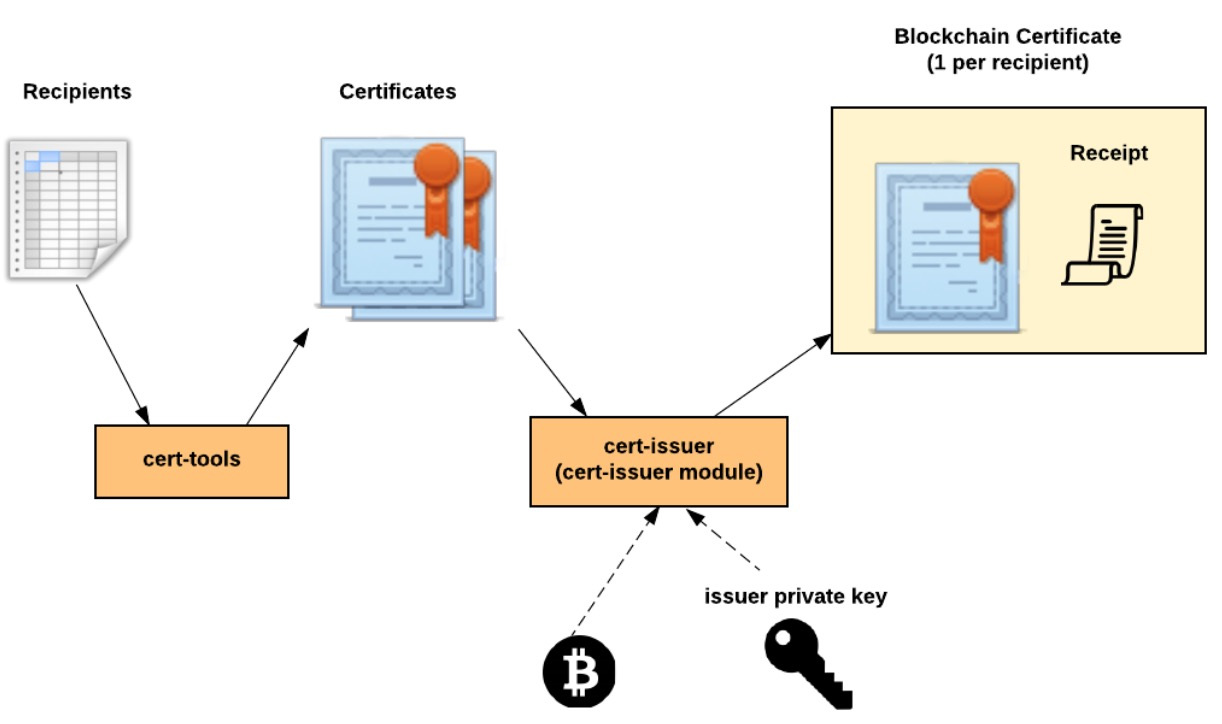
\includegraphics[width=\linewidth]{figures/blockcerts_arch.jpg}
  \caption{Blockcerts' certificate issuing architecture}
  \label{fig:blockcerts_arch}
\end{figure}

\begin{figure}[t!]
  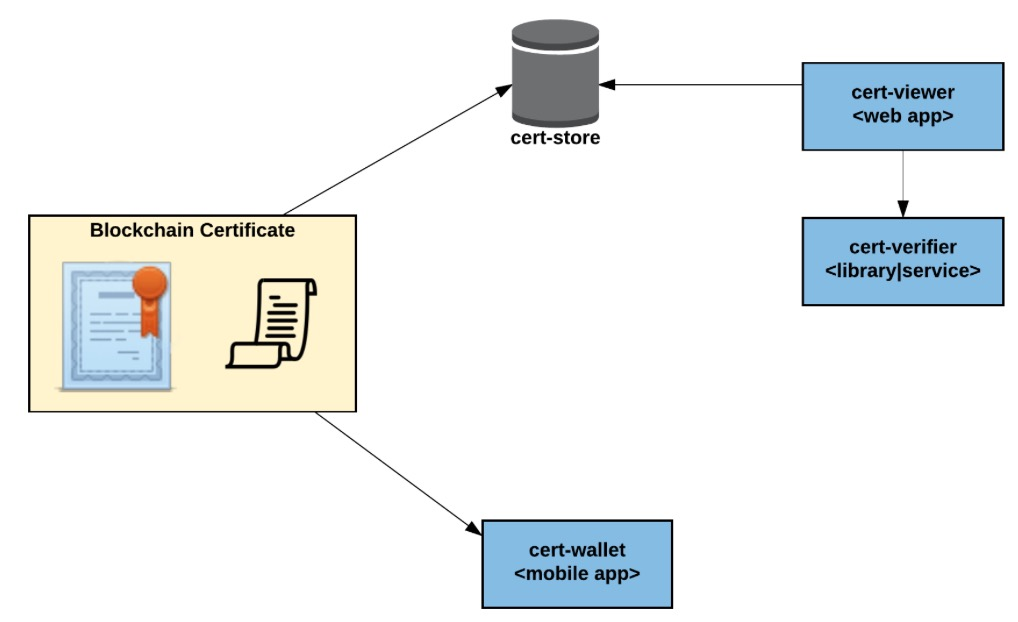
\includegraphics[width=\linewidth]{figures/cert_dist.jpg}
  \caption{Blockcerts' certificate distribution mechanism}
  \label{fig:blockcerts_dist}
\end{figure}

\subsubsection{Certificate Revocation}
\label{revoked}
One can think of a number of reasons a certificate may be revoked and as of now the way an Issuer can revoke a certificate it emitted if by publishing said certificate's ID on a Revoked Certificates List (each certificate has a field that says where to obtain the issuer's list of revoked certificates). This raises several problems, both from a technical perspective as well as a privacy one.


\subsubsection{Issues With the Current Certificate Revocation Model}
Blockcerts follows OpenBadges' specification for certificates revocation method. As of now, the way this is done is by having the issuer maintain a list of revoked certificates. An address to that list is provided on each issued certificate so that any party who wants to check the state of the certificate can do so by cross checking the certificate's ID with the list of revoked certificates.

This approach has been discussed in Blockcerts' forum and several problems have been highlighted:
\begin{itemize}
    \item \textbf{The issuer has total control over the certificate-} The certificate can only be revoked by the issuer (as he is the one in control of the revoked certificates list) and in the case of there being a need to revoke a batch of certificates, it has to be done one by one.
    \item \textbf{Verification relies on a third party-} Since the list is kept by the issuer, each time a party wants to verify a certificate it will have to communicate with the issuer. This creates a perpetual dependency between each certificate and its issuer which in turn defeats some of the purposes of using a blockchain, namely the capability of having a decentralised perpetual correct ledger. If the issuer ceases to exist there is no longer a way to revoke the certificates it once issued. This issue also ties up
    \item \textbf{Raises privacy concerns-} Each time the certificate revocation list is consulted on can assume the issuer can know about it (since it is the one hosting the list). This informs the issuer about the way the certificates are being used. Moreover, for each revoked certificate in that list there is a field in which the issuer can clarify the reason for the revocation, since the revoked certificates list is public, anyone can crawl those lists gathering information about revoked certificates.
  
\end{itemize}




\subsection{Ethereum}
The alt-coins seen in \ref{alt-coins} aim at solving some of bitcoin's shortcomings and lack of functionality, however they are highly optimised for one use case and lack flexibility to serve other purposes. Ethereum aims at solving this by offering smart-contracts \footnote{A script that runs in the blockchain} that have Turing completeness, effectively offering a state-machine that runs on the blockchain.

Ethereum is built on many of the same principles as Bitcoin. Is is a blockchain based system that can also serve as a cryptocurrency. It also uses a proof-of-work mechanism as consensus protocol, albeit with a difference, while Bitcoin's consensus protocol challenge lies on CPU power, Ethereum's lies on memory requirement. The goal of this different implementation is to make the network more democratic. One of the consequences of Bitcoin's consensus protocol was the creation of mining farms\footnote{Infrastructures provided with bitcoin mining specialised hardware} which resulted on an uneven distribution of the mining power among active nodes. Memory is something that is extremely optimised on pretty much every electronic device nowadays, much more than CPU power, so this measure should empower lighter miners to the detriment of more powerful ones.

\subsubsection{Turing Completeness}
Ethereum allows for developers to apply arbitrary logic to smart-contracts. Its transactions can be of one of two types.
\begin{itemize}
    \item Private: Are controlled by an ECC\footnote{Elliptic curve cryptography} private key and allow for currency transaction.
    \item Smart-contract: These are transactions controlled by the logic programed into a smart contract.
\end{itemize}
Both types of transactions can interact with one another (a private transaction can interact with a smart contract and the latter can also engage with a private transaction).
From a programing stand point, one can look at smart-contracts as objects in the Ethereum universe, these objects can interact with each other to fulfil any business rules required by an application.

A smart-contract has to define an upper limit of computing power it will use, this limit of computing power is knows as Gas. The amount of Gas a program has is what defines for how long it can be ran by Ethereum nodes. Gas costs money and miners are rewarded with that Gas. This condition is extremely important to stop programs that halted and malicious programs designed to enter an infinite loop. If a program runs and terminates successfully and does not spend all the Gas, the remainder is returned to the smart-contract, and can be used in future executions. On the other hand if a smart-contract runs out of Gas before ending its execution, all the changes made by the smart-contract are rolled back (to prevent inconsistent states) but the Gas is not returned to the smart-contract, it is given to the miners.






%%%%%%%%%%%%%%%%%%%%%%%%%%%%%%%%%%%%%%%%%%%%%

\subsection{IPFS}

IPFS (Interplanetary File System),\cite{Benet:2014vw}, is a peer-to-peer distributed file system.
Files are identified and linked to by a multiform cryptographic hash \footnote{The hash has information about the hash function used to generate it, as well as size and encoding} that is immutable and permanent. IPFS is extremely efficient in the way it handles data. Each node only needs to store the blocks it is interested in and when a node is searching for a file it queries the network for nodes who have that file.

IPFS keeps track of files by using a Merkle DAG\footnote{Directed Acyclic Graph},\cite{Merkle:1987jk}, a binary tree where each node is created by hashing its two child nodes, that allows for reliable verification of integrity in large data sets. This is the same data structure behind Git, Bitcoin and BitTorrent.

IPFS is built on top of IPLD, a protocol that allows for extreme flexibility in the way content is linked, allowing for instance an IPFS client to traverse into an Ethereum smart-contract and check the value of its variables - in a string based link, just like a file path in a Unix based system - without the need to run an Ethereum node.

IPFS is useful for a wide range of applications, one of them being blockchain. Storing data on a blockchain is inefficient and expensive. A user can store large amounts of data on IPFS and reference that data in blockchain transactions, by using the permanent and immutable hash.

Another useful feature of IPFS is that nodes need not to be connected to the backbone of the Internet in order to share files, they only need to be on the same network.

\section{Proposed Solution}
This body of work is going to address the Issuer hosted data dependence issue in two ways: 
\begin{enumerate}
    \item Dependency on Certificate Revocation
    \item Dependency on Certificate Storage
\end{enumerate}

To address the first we propose to leverage Ethereum's smart contracts to handle certificate revocations. This would allow us to add a lot of functionality and flexibility to the system.

To address the second we propose a new method to store certificates that relies on the distributed file system, IPFS, by referencing each certificate with a permanent immutable link.


\subsection{Architecture}
It is important to mention that this would not automatically solve the issue of dependence on a specific blockchain. That is outside of the scope of this work. There is a proposal to how that should be address and it points towards there being an implementation per blockchain (one for Bitcoin, one for Ethereum) and then having Blockcerts interface with them. So even though this does not make Blockcerts blockchain agnostic, it contributes to the effort of having an implementation per blockchain. This is illustrated in \ref{fig:scope}



\begin{figure}[t!]
  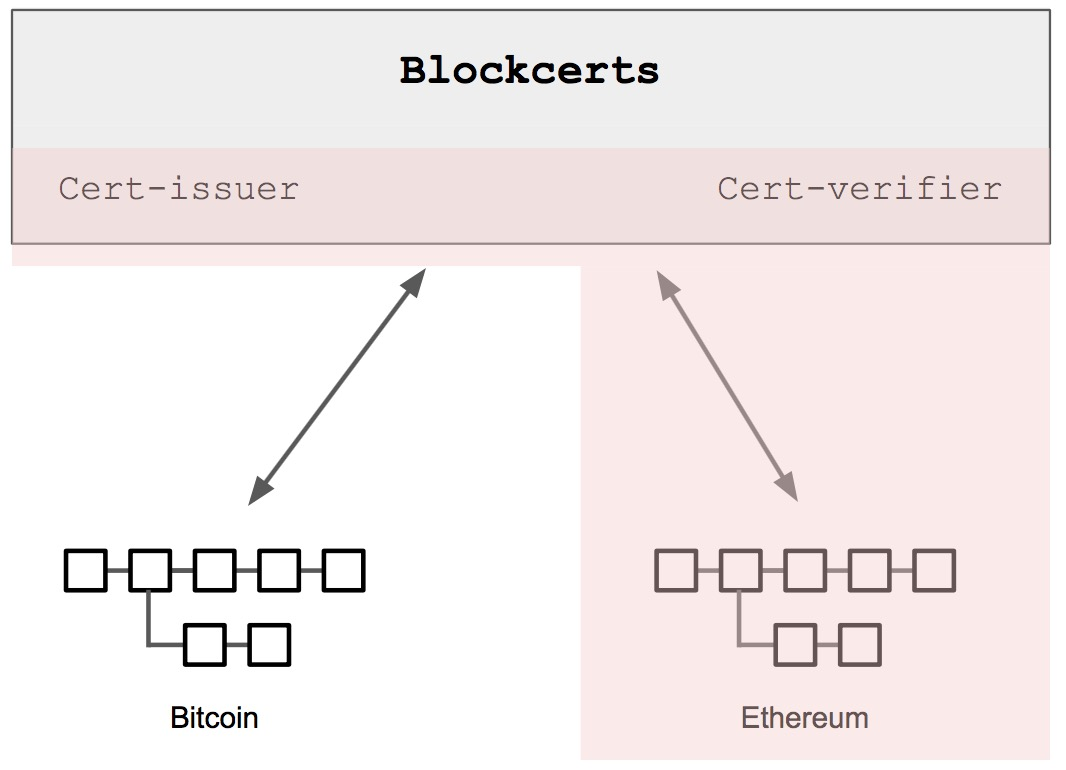
\includegraphics[width=\linewidth]{figures/arch.jpg}
  \caption{Scope of this work. We will focus on developing an Ethereum smart-contract's implementation for certificate revocation}
  \label{fig:scope}
\end{figure}
\subsection{Functionalities}
Our implementation will support the following functionalities, which were suggested in  Blockcerts' forum as desirable features, to the certificate revocation mechanism:
\begin{itemize}
    \item \textbf{Revocation by the Issuer:} Just like it currently exists.
    \item \textbf{Revocation by the Receiver:} A new functionality, not supported by revoked certificates list, which gives the receiver full control over the certificates it may hold. It is legitimate to imagine a scenario where a receiver no longer wants to be associated with a given Issuer.
    \item \textbf{Revocation by a third-party:} Another new feature which will allow a third-party, authorised by the Issuer and Receiver, to revoke a certificate.
    \item \textbf{Revocation by a combination of Issuer, Receiver and third-party}
    \item \textbf{Temporary revocation:} A unique feature of a smart-contract based approach to this is that the revocation status can be changed over time. This will allow for temporary revocation status that can be triggered by a programmable action (for instance, a certificate can be revoked if a receiver fails to pay a pre-accorded monthly fee).
    \item \textbf{Batch revocation-} This implementation will allow for an easy batch revocation.
    \item \textbf{Store certificate on IPFS:} Issuers will have the ability to directly store the certificate on IPFS. They can then use the IPFS link to share the file with the recipients.
\end{itemize}

\subsection{Remove Issuers' Dependency on Certificate Revocation}
There are several ideas on how to solve this. One proposed approach is to use Bitcoin's unspent transaction outputs (UTXOs). By assigning and UTXO to a certificate the way to revoke said certificate would be to perform a transaction that utilised that UTXO, which would render the unspent transaction output, spent. This approach solves all the problems that come with the Revoked Certificates List. The certificate can now be revoked by more than one party (by implementing a Bitcoin smart-contract with multi-signature), the verification no longer requires a third party, as it can be made entirely relying on the Bitcoin blockchain and privacy concerns are no longer an issue (certificate revocation reasons are still public but are recorded i individual files, rather than being all together on a list).

Even though this mechanism would solve the problems with the existing system, it also adds problems of its own:
\begin{itemize}
    \item \textbf{Provides little functionality-} Once revoked the certificate can no longer the valid. A desirable feature on a system such as this one would be the ability to freeze certificates, that same way bank accounts can temporarily be frozen.
    \item \textbf{It is Bitcoin specific-} Even though Blockcerts' current implementation is made on top of the Bitcoin blockchain, the long-term goal is for it to be blockchain agnostic. For that reason, creating a dependency on the Bitcoin blockchain is not a desirable feature.
    \item \textbf{The cost of revoking batches if very high-} It is legitimate to assume that sometimes there will be the need to revoke a batch of certificates. With this approach this would require one transaction per revoked certificate. Since each transaction has a cost associated with it, revoking a whole batch of certificates would make the revoking cost grow linearly with the number of certificates in the batch.
\end{itemize}

\subsubsection{Integration With Ethereum}
Ethereum offers a great set of tools that will enable us to add aforementioned functionalities to the system. Since it's Turing complete and has support for familiar programing languages, its smart-contracts can be programmed almost like normal applications.

The revocation status of a given certificate can be maintained as a variable in a smart-contract. Certificates revocation status can be accessed individually or as a batch. A simple architecture to support this would be to have a smart-contract per batch of certificates. 

Implementing an Ethereum smart-contracts solution for certificate revocation will require changes to some of Blockcerts' components (refer to Figure \ref{fig:blockcerts_arch}):
\begin{itemize}
    \item \textbf{Blockcerts Schema-} The Blockcerts schema defines the fields and schema a certificate must have in order to be Blockcerts compliant. Currently one of the required fields is the Revocation List, which contains either an HTTP URI\footnote{Uniform Resource Identifier} pointing towards the Issuer's revoked certificates list or an embedded array of revoked certificates. This schema will be extended in order to contain a URI pointing towards that specific certificate's status, that URI can point to an Ethereum smart-contract, to a Bitcoin UTXO, depending on the implementation (this because even though we will be procuring an Ethereum implementation, the goal is to make Blockcerts certificate revocation function with any blockchain that can support the functionality).
    
    \item \textbf{Cert-Tools-} This component receives inputs\footnote{Data relevant to the issuing of the certificate} from the Issuer and outputs a Blockcerts compliant certificate.It will be required to extend this component to comply with the schema changes proposed above.
    \item \textbf{Cert-Verifier-} The Cert-verifier is responsible for checking the integrity, authenticity and revocation status of a given certificate. This component will also be extended to account for the new revocation status verification mechanism. In this case it will check the revocation status in the Ethereum smart-contract.
\end{itemize}

\subsection{Remove Dependencies From Issuers' Certificate Storage}
In the current implementation of blockcerts, the Issuers are the ones responsible for keeping a copy of the certificates. This not only creates a single point of failure but also, just like the revoked certificates list case, creates a perpetual dependency on the Issuer. IPFS offers an efficient distributed storage solution. Contents are addressed by unique links that are permanent and immutable.

Blockcerts provides a reference mechanism for Issuers to store their issued certificates, Cert-store, which is implemented in MongoDB. They do make clear, however, that this implementation is not part of the standard and that any Issuer can have different approaches to how they store their certificates. The only required aspect is that the certificates can be retrieved via a URL, and IPFS complies with that.

In order to accomplish certificate storage on IPFS we propose to change the Cert-store and the Cert-viewer.
\begin{itemize}
    \item \textbf{Cert-Store:} This is the application that Issuers can use to store their issued certificates. We want to implement this application in a way that stores certificates on IPFS.
    \item \textbf{Cert-viewer:} This application is used to retrieve certificates when provided with a URL. We need to extend this application in order to support IPFS' URLs.
\end{itemize}


\section{Evaluation}
\label{sec:evaluation}
The value of this work is directly related to the importance it will have as an improvement Blockcerts' current system. To that end we intend to evaluate the system in three components:

\begin{itemize}
    \item \textbf{Revocation Cost:} There is an associated cost with every transaction.We are going to create a private Ethereum blockchain and review the transaction outputs, which will give us information about the cost of each revocation.
    \item \textbf{Revocation Performance:} Blockchains are knows for its low throughput and Ethereum is no exception. While revoking individual certificates should not be an issue, revoking batches might by. To that end we will deploy our system in the Ethereum blockchain and test the performance.
    \item \textbf{Functionality:} Test the new functionalities on the newly extended applications.
\end{itemize}

\subsection{Performance Evaluation}

\section{Scheduling of Future Work}
\label{sec:fwork}

Future work is scheduled as follows:

\begin{itemize}
\item \textbf{September 15 - December 10} 
    \begin{itemize}
        \item Detailed design specifications, implementation and documentation.
        \item Submit the software to Blockcerts' Github repository as a pull request.
    \end{itemize}
\item \textbf{December 10 - January 5}
    \begin{itemize}
        \item Receive community feedback and improve the solution. 
        \item Start writing a technical paper describing the solution. 
        \item Start system testing and evaluation.
    \end{itemize}
\item \textbf{January 5 - February 15} 
    \begin{itemize}
        \item Complete testing and evaluation
        \item Conclude technical paper
        \item Finalise the writing the dissertation.
    \end{itemize}
\item \textbf{February 20} Deliver the MSc dissertation.

\end{itemize}

\section{Conclusions}
\label{sec:conclusions}



\bibliographystyle{splncs}
\bibliography{relatorio}

\acrodef{IDK}{I Don't Know}

\end{document}
